\section{Results}\label{Sec:Results}

\subsection{Empirical confidence regions}

Tables~\ref{Tab:Points1k} and~\ref{Tab:Points50k} list the coordinates in the $H\times C$ plane
of the emblematic point $\bm P'$ and of the four points $\bm P_1,\bm P_2,\bm P_3,\bm P_4$ that define the confidence regions at \SI{90}{\percent}, \SI{95}{\percent}, \SI{99}{\percent}, and \SI{99.9}{\percent}, 
for $D=3,4,5,6$ and $N=1000,50000$, .
The points are presented counterclockwise, starting with the one with the largest complexity. 

\begin{comment}
\begin{table}[hbt]
\caption{Coordinates in the $H\times C$ plane of the emblematic series and the points that define the confidence regions at \SI{90}{\percent}, \SI{95}{\percent}, \SI{99}{\percent}, and \SI{99.9}{\percent} for $D=3,4,5,6$ and $N=1000,50000$}\label{Tab:Points}
\centering
\begin{tabular}{rcllllllll}
\toprule
& & \multicolumn{8}{c}{$N$}\\ \cmidrule(lr){3-10}
& & \multicolumn{4}{c}{$1000$} & \multicolumn{4}{c}{$50000$}\\ \cmidrule(lr){3-6} \cmidrule(lr){7-10}
$D$ & Point & \SI{90}{\percent} & \SI{95}{\percent} & \SI{99}{\percent} & \SI{99.9}{\percent} & \SI{90}{\percent} & \SI{95}{\percent} & \SI{99}{\percent} & \SI{99.9}{\percent}\\ \cmidrule(lr){3-3} \cmidrule(lr){4-4} \cmidrule(lr){5-5} \cmidrule(lr){6-6} \cmidrule(lr){7-7} \cmidrule(lr){8-8} \cmidrule(lr){9-9} \cmidrule(lr){10-10}
$3$ & $\bm P'$ & \multicolumn{4}{c}{$h',c'$} & \multicolumn{4}{c}{$h',c'$}\\
& $\bm P_1$ & $(0.9973334, 0.0025601)$ & $(0.9967311, 0.0031343)$ & $(0.9953009, 0.0045054)$ & $(0.9931825, 0.0065387)$ & $(0.9999489, \num[scientific-notation=true]{5.06e-05})$ & $(0.9999384, \num[scientific-notation=true]{6.11e-05})$ & $(0.9999079, \num[scientific-notation=true]{9.11e-05})$ & $(0.9998625, 0.0001361)$\\
& $\bm P_2$ & $(0.9974047, 0.0026304)$ & $(0.9968219, 0.0032238)$ & $(0.9954349, 0.0046375)$ & $(0.9933704, 0.006724)$ & $(0.9999487, \num[scientific-notation=true]{5.04e-05})$ & $(0.9999382, \num[scientific-notation=true]{6.09e-05})$ & $(0.9999077, \num[scientific-notation=true]{9.09e-05})$ & $(0.9998622, 0.0001358)$\\
& $\bm P_3$ & $(0.9999497, 0)$ & $(0.9999398, 0)$ & $(0.9999203, 0)$ & $(0.9998925, 0)$ & $(0.9999998, \num[scientific-notation=true]{4e-07})$ & $(0.9999994, \num[scientific-notation=true]{9e-07})$ & $(0.9999982, \num[scientific-notation=true]{2e-06})$ & $(0.9999973, \num[scientific-notation=true]{3e-06})$\\
& $\bm P_4$ & $(1, \num[scientific-notation=true]{5.17e-05})$ & $(1, \num[scientific-notation=true]{6.12e-05})$ & $(1, \num[scientific-notation=true]{8.45e-05})$ & $(1, 0.0001104)$ & $(0.9999996, \num[scientific-notation=true]{2e-07})$ & $(0.9999991, \num[scientific-notation=true]{7e-07})$ & $(0.999998, \num[scientific-notation=true]{1.8e-06})$ & $(0.999997, \num[scientific-notation=true]{2.7e-06})$\\ \midrule
$4$ & $\bm P'$ & \multicolumn{4}{c}{$h',c'$} & \multicolumn{4}{c}{$h',c'$}\\
& $\bm P_1$ & $(0.994364, 0.0081246)$ & $(0.9937138, 0.0089796)$ & $(0.9922575, 0.0108947)$ & $(0.9902578, 0.0135243)$ & $(0.9999684, \num[scientific-notation=true]{3.98e-05})$ & $(0.9999725, \num[scientific-notation=true]{3.44e-05})$ & $(0.9999783, \num[scientific-notation=true]{2.68e-05})$ & $(0.9999833, \num[scientific-notation=true]{2.02e-05})$ \\
& $\bm P_2$ & $(0.9939234, 0.0075452)$ & $(0.9932534, 0.0083741)$ & $(0.9917308, 0.0102022)$ & $(0.9897312, 0.0128318)$ & $(0.9999696, \num[scientific-notation=true]{4.13e-05})$ & $(0.9999737, \num[scientific-notation=true]{3.6e-05})$ & $(0.9999795, \num[scientific-notation=true]{2.83e-05})$ & $(0.9999845, \num[scientific-notation=true]{2.18e-05})$ \\
& $\bm P_3$ & $(0.9994791, 0.0013982)$ & $(0.9991609, 0.0018166)$ & $(0.9987924, 0.0023012)$ & $(0.9985727, 0.0025901)$ & $(0.9998075, 0.0002508)$ & $(0.9998506, 0.0001942)$ & $(0.9998756, 0.0001615)$ & $(0.9998889, 0.000144)$ \\
& $\bm P_4$ & $(0.9990385, 0.0008188)$ & $(0.9987005, 0.0012111)$ & $(0.9982658, 0.0016087)$ & $(0.9980461, 0.0018976)$ & $(0.9998087, 0.0002524)$ & $(0.9998518, 0.0001958)$ & $(0.9998768, 0.000163)$ & $(0.9998901, 0.0001456)$ \\ \midrule
$5$ & $\bm P'$ & \multicolumn{4}{c}{$h',c'$} & \multicolumn{4}{c}{$h',c'$}\\
& $\bm P_1$ & $(0.9811818, 0.0321294)$ & $(0.9801289, 0.0340045)$ & $(0.977917, 0.0377295)$ & $(0.9753326, 0.0425299)$ & $(0.9998172, 0.0003232)$ & $(0.9998259, 0.0003075)$ & $(0.9998428, 0.0002774)$ & $(0.9998573, 0.0002517)$ \\
& $\bm P_2$ & $(0.9827429, 0.0350291)$ & $(0.9817117, 0.0369446)$ & $(0.9796031, 0.0408613)$ & $(0.9770187, 0.0456617)$ & $(0.9998194, 0.0003273)$ & $(0.9998282, 0.0003116)$ & $(0.999845, 0.0002814)$ & $(0.9998593, 0.0002553)$ \\
& $\bm P_3$ & $(0.9919707, 0.0120896)$ & $(0.9909376, 0.0139279)$ & $(0.9898161, 0.0156277)$ & $(0.9892599, 0.0166608)$ & $(0.9994812, 0.0009246)$ & $(0.9996371, 0.0006455)$ & $(0.9996703, 0.0005862)$ & $(0.9996884, 0.000554)$ \\
& $\bm P_4$ & $(0.9935319, 0.0149893)$ & $(0.9925204, 0.016868)$ & $(0.9915021, 0.0187595)$ & $(0.9909459, 0.0197926)$ & $(0.9994834, 0.0009286)$ & $(0.9996394, 0.0006495)$ & $(0.9996725, 0.0005901)$ & $(0.9996904, 0.0005576)$ \\ \midrule
$6$ & $\bm P'$ & \multicolumn{4}{c}{$h',c'$} & \multicolumn{4}{c}{$h',c'$}\\
& $\bm P_1$ & $(0.9121895, 0.2201993)$ & $(0.9105951, 0.2239294)$ & $(0.9105951, 0.2239294)$ & $(0.9077672, 0.2305874)$ & $(0.9990169, 0.002336)$ & $(0.9990368, 0.002288)$ & $(0.9990736, 0.0021997)$ & $(0.9991069, 0.0021197)$ \\
& $\bm P_2$ & $(0.9146048, 0.2260776)$ & $(0.9130413, 0.2298829)$ & $(0.9130413, 0.2298829)$ & $(0.9102595, 0.2366531)$ & $(0.9990249, 0.0023554)$ & $(0.9990449, 0.0023074)$ & $(0.9990817, 0.0022191)$ & $(0.999115, 0.0021392)$ \\
& $\bm P_3$ & $(0.9443868, 0.1418373)$ & $(0.9419202, 0.1476904)$ & $(0.9396577, 0.1531967)$ & $(0.9383611, 0.1561279)$ & $(0.9978983, 0.0050219)$ & $(0.998714, 0.0030633)$ & $(0.998765, 0.0029407)$ & $(0.9987884, 0.0028845)$ \\
& $\bm P_4$ & $(0.9468021, 0.1477156)$ & $(0.9443663, 0.1536439)$ & $(0.9421039, 0.1591502)$ & $(0.9408534, 0.1621937)$ & $(0.9979064, 0.0050413)$ & $(0.998722, 0.0030827)$ & $(0.9987731, 0.0029601)$ & $(0.9987965, 0.0029039)$ \\ \bottomrule
\end{tabular}
\end{table}
\end{comment}

\begin{table}[hbt]
	\caption{Coordinates in the $H\times C$ plane of the emblematic series and the points that define the confidence regions at \SI{90}{\percent}, \SI{95}{\percent}, \SI{99}{\percent}, and \SI{99.9}{\percent} for $D=3,4,5,6$ and $N=1000$}\label{Tab:Points1k}
	\centering
	\begin{tabular}{rccccc}
		\toprule
		%& & \multicolumn{4}{c}{$N$}\\ 
		%\cmidrule(lr){3-6}
		& & \multicolumn{4}{c}{$N = 1000$}\\ 
		\cmidrule(lr){3-6} 
		$D$ & Point & \SI{90}{\percent} & \SI{95}{\percent} & \SI{99}{\percent} & \SI{99.9}{\percent}\\ 
		\cmidrule(lr){3-3} 
		\cmidrule(lr){4-4} 
		\cmidrule(lr){5-5} 
		\cmidrule(lr){6-6} 
		$3$ & $\bm P'$ & \multicolumn{4}{c}{$(0.9992089,0.0007800)$}\\
		& $\bm P_1$ & $(0.9973334, 0.0025601)$ & $(0.9967311, 0.0031343)$ & $(0.9953009, 0.0045054)$ & $(0.9931825, 0.0065387)$\\
		& $\bm P_2$ & $(0.9974047, 0.0026304)$ & $(0.9968219, 0.0032238)$ & $(0.9954349, 0.0046375)$ & $(0.9933704, 0.006724)$\\
		& $\bm P_3$ & $(0.9999497, 0)$ & $(0.9999398, 0)$ & $(0.9999203, 0)$ & $(0.9998925, 0)$\\
		& $\bm P_4$ & $(1, \num[scientific-notation=true]{5.17e-05})$ & $(1, \num[scientific-notation=true]{6.12e-05})$ & $(1, \num[scientific-notation=true]{8.45e-05})$ & $(1, 0.0001104)$\\ 
		\midrule
		$4$ & $\bm P'$ & \multicolumn{4}{c}{$(0.9967032, 0.0043297)$} \\
		& $\bm P_1$ & $(0.994364, 0.0081246)$ & $(0.9937138, 0.0089796)$ & $(0.,9922575 0.0108947)$ & $(0.9902578, 0.0135243)$\\
		& $\bm P_2$ & $(0.9939234, 0.0075452)$ & $(0.9932534, 0.0083741)$ & $(0.9917308, 0.0102022)$ & $(0.9897312, 0.0128318)$\\
		& $\bm P_3$ & $(0.9994791, 0.0013982)$ & $(0.9991609, 0.0018166)$ & $(0.9987924, 0.0023012)$ & $(0.9985727, 0.0025901)$\\
		& $\bm P_4$ & $(0.9990385, 0.0008188)$ & $(0.9987005, 0.0012111)$ & $(0.9982658, 0.0016087)$ & $(0.9980461, 0.0018976)$\\ 
		\midrule
		$5$ & $\bm P'$ & \multicolumn{4}{c}{$(0.9864873, 0.0245632)$}\\
		& $\bm P_1$ & $(0.9811818, 0.0321294)$ & $(0.9801289, 0.0340045)$ & $(0.977917, 0.0377295)$ & $(0.9753326, 0.0425299)$\\
		& $\bm P_2$ & $(0.9827429, 0.0350291)$ & $(0.9817117, 0.0369446)$ & $(0.9796031, 0.0408613)$ & $(0.9770187, 0.0456617)$\\
		& $\bm P_3$ & $(0.9919707, 0.0120896)$ & $(0.9909376, 0.0139279)$ & $(0.9898161, 0.0156277)$ & $(0.9892599, 0.0166608)$\\
		& $\bm P_4$ & $(0.9935319, 0.0149893)$ & $(0.9925204, 0.016868)$ & $(0.9915021, 0.0187595)$ & $(0.9909459, 0.0197926)$\\ 
		\midrule
		$6$ & $\bm P'$ & \multicolumn{4}{c}{$(0,9296429, 0.1841438)$}\\
		& $\bm P_1$ & $(0.9121895, 0.2201993)$ & $(0.9105951, 0.2239294)$ & $(0.9105951, 0.2239294)$ & $(0.9077672, 0.2305874)$\\
		& $\bm P_2$ & $(0.9146048, 0.2260776)$ & $(0.9130413, 0.2298829)$ & $(0.9130413, 0.2298829)$ & $(0.9102595, 0.2366531)$\\
		& $\bm P_3$ & $(0.9443868, 0.1418373)$ & $(0.9419202, 0.1476904)$ & $(0.9396577, 0.1531967)$ & $(0.9383611, 0.1561279)$\\
		& $\bm P_4$ & $(0.9468021, 0.1477156)$ & $(0.9443663, 0.1536439)$ & $(0.9421039, 0.1591502)$ & $(0.9408534, 0.1621937)$\\ 
		\bottomrule
	\end{tabular}
\end{table}


\begin{table}[hbt]
	\caption{Coordinates in the $H\times C$ plane of the emblematic series and the points that define the confidence regions at \SI{90}{\percent}, \SI{95}{\percent}, \SI{99}{\percent}, and \SI{99.9}{\percent} for $D=3,4,5,6$ and $N=50000$}\label{Tab:Points50k}
	\centering
	\begin{tabular}{rccccc}
		\toprule
		%& & \multicolumn{4}{c}{$N$}\\ 
		%\cmidrule(lr){3-6}
		& & \multicolumn{4}{c}{$N = 50000$}\\ 
		\cmidrule(lr){3-6} 
		$D$ & Point & \SI{90}{\percent} & \SI{95}{\percent} & \SI{99}{\percent} & \SI{99.9}{\percent}\\ 
		\cmidrule(lr){3-3} 
		\cmidrule(lr){4-4} 
		\cmidrule(lr){5-5} 
		\cmidrule(lr){6-6} 
		$3$ & $\bm P'$ & \multicolumn{4}{c}{$(0.9999853, \num[scientific-notation=true]{1.45e-05})$}\\
		& $\bm P_1$ & $(0.9999489, \num[scientific-notation=true]{5.06e-05})$ & $(0.9999384, \num[scientific-notation=true]{6.11e-05})$ & $(0.9999079, \num[scientific-notation=true]{9.11e-05})$ & $(0.9998625, 0.0001361)$\\
		& $\bm P_2$ & $(0.9999487, \num[scientific-notation=true]{5.04e-05})$ & $(0.9999382, \num[scientific-notation=true]{6.09e-05})$ & $(0.9999077, \num[scientific-notation=true]{9.09e-05})$ & $(0.9998622, 0.0001358)$\\
		& $\bm P_3$ & $(0.9999998, \num[scientific-notation=true]{4e-07})$ & $(0.9999994, \num[scientific-notation=true]{9e-07})$ & $(0.9999982, \num[scientific-notation=true]{2e-06})$ & $(0.9999973, \num[scientific-notation=true]{3e-06})$\\
		& $\bm P_4$ & $(0.9999996, \num[scientific-notation=true]{2e-07})$ & $(0.9999991, \num[scientific-notation=true]{7e-07})$ & $(0.999998, \num[scientific-notation=true]{1.8e-06})$ & $(0.999997, \num[scientific-notation=true]{2.7e-06})$\\ \midrule
		$4$ & $\bm P'$ & \multicolumn{4}{c}{$(0.9999394, \num[scientific-notation=true]{7.94e-05})$}\\
		& $\bm P_1$ & $(0.9999684, \num[scientific-notation=true]{3.98e-05})$ & $(0.9999725, \num[scientific-notation=true]{3.44e-05})$ & $(0.9999783, \num[scientific-notation=true]{2.68e-05})$ & $(0.9999833, \num[scientific-notation=true]{2.02e-05})$ \\
		& $\bm P_2$ & $(0.9999696, \num[scientific-notation=true]{4.13e-05})$ & $(0.9999737, \num[scientific-notation=true]{3.6e-05})$ & $(0.9999795, \num[scientific-notation=true]{2.83e-05})$ & $(0.9999845, \num[scientific-notation=true]{2.18e-05})$ \\
		& $\bm P_3$ & $(0.9998075, 0.0002508)$ & $(0.9998506, 0.0001942)$ & $(0.9998756, 0.0001615)$ & $(0.9998889, 0.000144)$ \\
		& $\bm P_4$ & $(0.9998087, 0.0002524)$ & $(0.9998518, 0.0001958)$ & $(0.9998768, 0.000163)$ & $(0.9998901, 0.0001456)$ \\ \midrule
		$5$ & $\bm P'$ & \multicolumn{4}{c}{$(0.9997616, 0.0004264)$}\\
		& $\bm P_1$ & $(0.9998172, 0.0003232)$ & $(0.9998259, 0.0003075)$ & $(0.9998428, 0.0002774)$ & $(0.9998573, 0.0002517)$ \\
		& $\bm P_2$ & $(0.9998194, 0.0003273)$ & $(0.9998282, 0.0003116)$ & $(0.999845, 0.0002814)$ & $(0.9998593, 0.0002553)$ \\
		& $\bm P_3$ & $(0.9994812, 0.0009246)$ & $(0.9996371, 0.0006455)$ & $(0.9996703, 0.0005862)$ & $(0.9996884, 0.000554)$ \\
		& $\bm P_4$ & $(0.9994834, 0.0009286)$ & $(0.9996394, 0.0006495)$ & $(0.9996725, 0.0005901)$ & $(0.9996904, 0.0005576)$ \\ \midrule
		$6$ & $\bm P'$ & \multicolumn{4}{c}{$(0.9989108, 0.0026093)$}\\
		& $\bm P_1$ & $(0.9990169, 0.002336)$ & $(0.9990368, 0.002288)$ & $(0.9990736, 0.0021997)$ & $(0.9991069, 0.0021197)$ \\
		& $\bm P_2$ & $(0.9990249, 0.0023554)$ & $(0.9990449, 0.0023074)$ & $(0.9990817, 0.0022191)$ & $(0.999115, 0.0021392)$ \\
		& $\bm P_3$ & $(0.9978983, 0.0050219)$ & $(0.998714, 0.0030633)$ & $(0.998765, 0.0029407)$ & $(0.9987884, 0.0028845)$ \\
		& $\bm P_4$ & $(0.9979064, 0.0050413)$ & $(0.998722, 0.0030827)$ & $(0.9987731, 0.0029601)$ & $(0.9987965, 0.0029039)$ \\ \bottomrule
	\end{tabular}
\end{table}

Fig.~\ref{fig:HC-PCA} shows the results for $T = 50000$ and $D = 3,6$ in the new principal components space, along with the quantiles of order $\SI{90}{\percent}$, $\SI{95}{\percent}$, $\SI{99}{\percent}$, and $\SI{99.9}{\percent}$.
We also show the projection of the $H \times C$ plane boundaries in this space, as well the median of each data set, the latter being represented as red dots.

\begin{figure}[hbt]
	\centering
	\subfloat[Points in the Principal Components plane for for $D=3$]{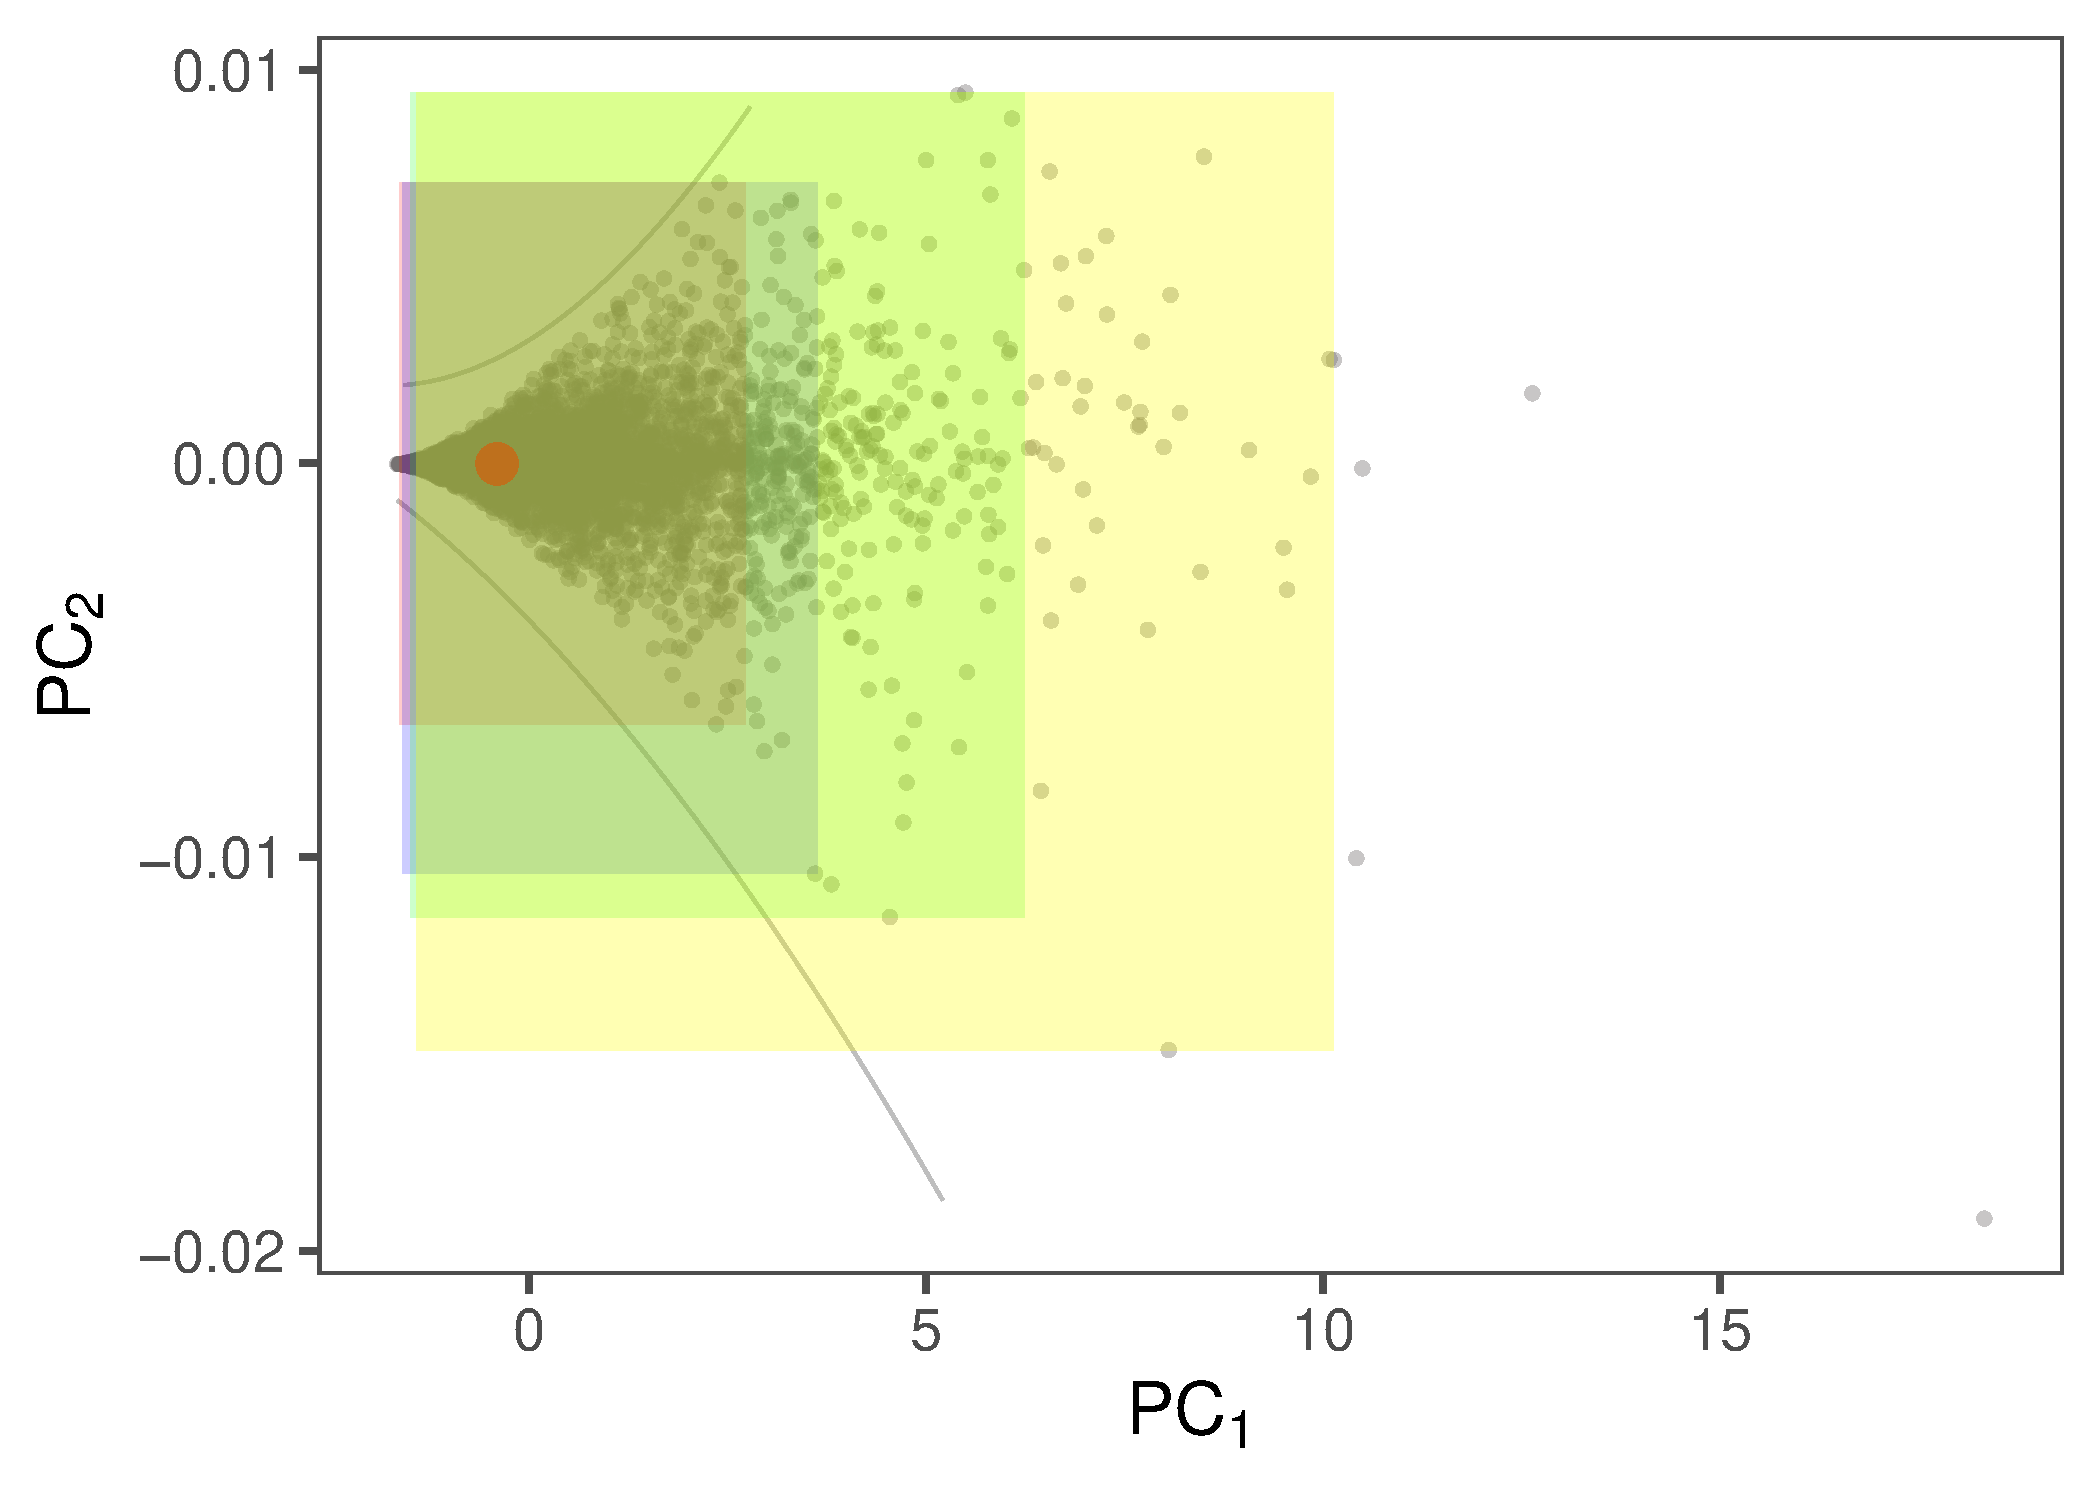
\includegraphics[width=.49\linewidth]{Figures/HC-PCA-Trozos-D3N50k}}
	\subfloat[Points in the Principal Components plane for for $D=6$]{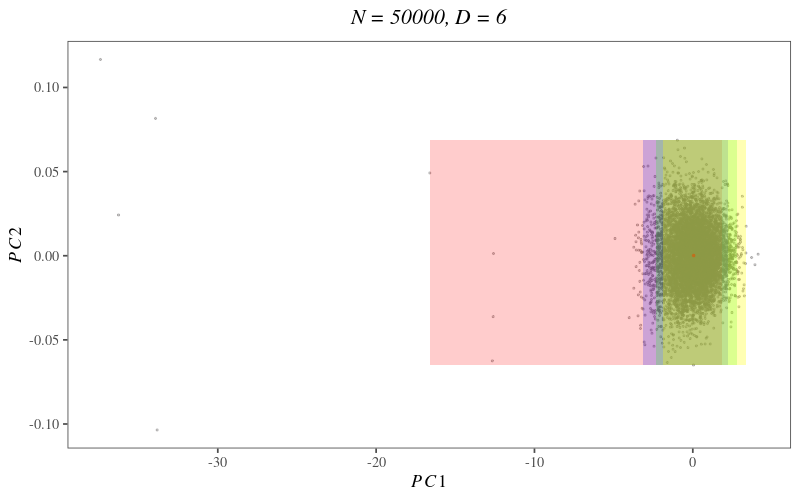
\includegraphics[width=.49\linewidth]{Figures/HC-PCA-Trozos-D6N50k}}
	\caption{Representation of true random white noise sequences of length $T = 50000$ in the PCA space for $D = 3$ and $D = 6$, and the quantiles of $\SI{90}{\percent}$, $\SI{95}{\percent}$, $\SI{99}{\percent}$, and $\SI{99.9}{\percent}$.}
	\label{fig:HC-PCA}
\end{figure} 

The confidence regions exceed the $H \times C$ boundaries, but this issue does not compromise the test's size since no points can be observed outside such boundaries.

Fig.~\ref{fig:HC-PCA} also shows that the data are not evenly distributed among the axes of the first principal component.
They tend to concentrate close to the point that corresponds to $(1,0)$ in the $H\times C$ plane.
As we use order statistics to define the confidence regions, this issue is also of little relevance for our results.
Moreover, Fig.~\ref{fig:PCA-Hist} shows that such asymmetry diminishes when the embedding dimension $D$ increases.

\begin{figure}[hbt]
	\centering
	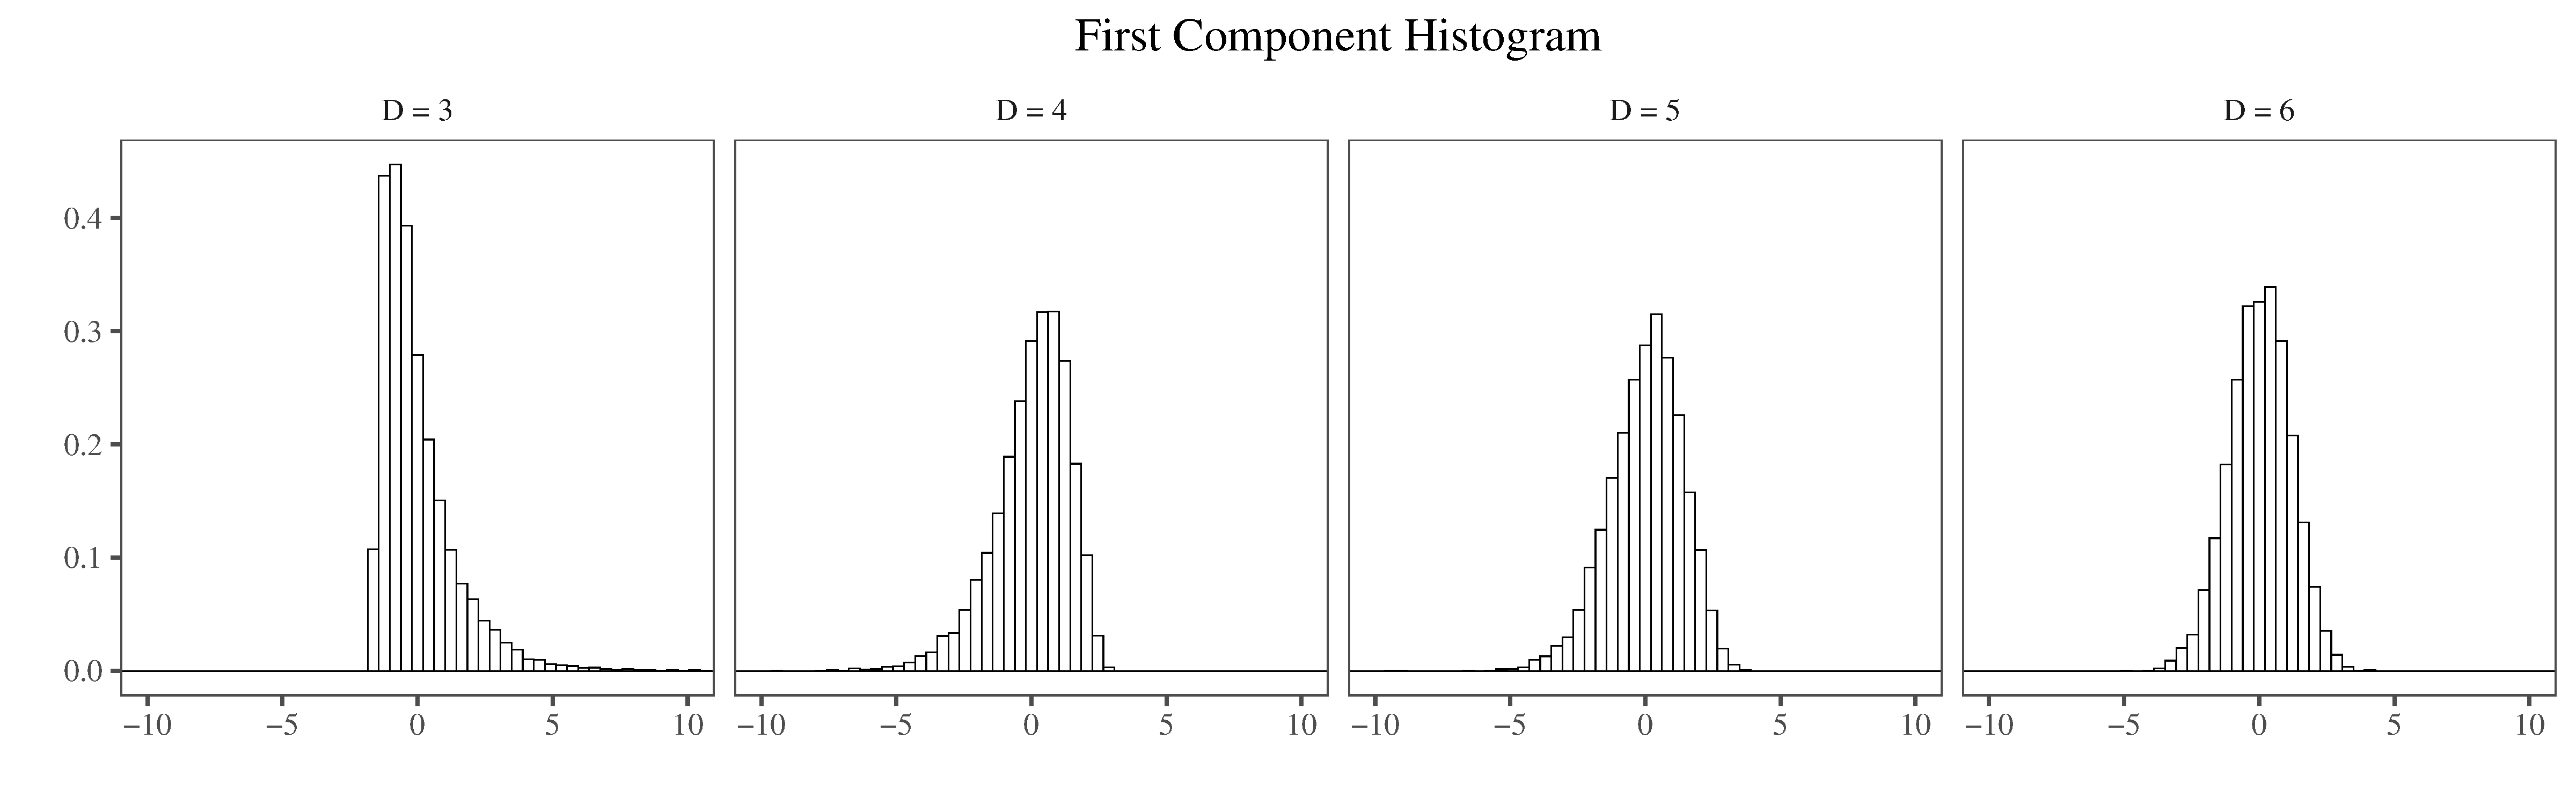
\includegraphics[width=\linewidth]{PCA-hist-50k}
	\caption{Histograms of the first principal component for $D=3,4,5,6$}
	\label{fig:PCA-Hist}
\end{figure}

\subsection{Test Size}

We assessed the size of the test by contrasting $100$ new TWNRS for each situation of $D=3,4,5,6$ and of $\alpha=0.01,0.05$.
Table~\ref{tab:result1} and Fig.~\ref{fig:RNG} 
show the results.

On the one hand, long series ($T=50000$) present a good size for every embedding dimension.
On the other hand, short series ($T=1000$) exhibit only one situation with a noticeable divergence between the expected and the observed size: the test rejects \SI{13}{\percent} of the $100$ series when $D=6$. 
In contrast, we expected \SI{1}{\percent} of rejection.
This might be because, in this case, the condition $D!\ll T$ is not respected.
Notice that the wrongly rejected TWNRS are all close to the point $(1,0)$.

%
%For large series, $T = 50000$, the closest although we observed a small drop in the percentage of data present in the region with $\SI{99}{\percent}$ confidence, there was a significant increase in points in the region with $\SI{95}{\percent}$ confidence, showing between $\SI{90}{\percent}$ and $\SI{88}{\percent}$ of the points when we vary the embedding dimension.
%
%For short series, $T = 1000$, and $D = 3$ 
%the conficence region at $\SI{99}{\percent}$ contains exactly $\SI{99}{\percent}$.
%
%On the other hand, there was a very large loss of points located in the region with $\SI{95}{\percent}$ confidence as the dimension increased.
%A reasonable explanation for this event is given in the choice of the parameter itself.
%It is known by definition that $D! \ll N$, which does not happen for such a sample size, thus presenting many missing patterns that lead to an unrepresentative probability distribution.

\begin{table}[hbt]
	\centering
	\caption{Empirical sizes of the test}
	\label{tab:result1}
	\begin{tabular}{*{3}rr}
		\toprule
		\multicolumn{1}{c}{$N$} & \multicolumn{1}{c}{$D$} & \multicolumn{1}{c}{\SI{95}{\percent}} & \multicolumn{1}{c}{\SI{99}{\percent}}\\
		%& $p$-value\\
		\cmidrule(lr){1-1}
		\cmidrule(lr){2-2}
		\cmidrule(lr){3-3}
		\cmidrule(lr){4-4}
		1000 & 3 & $0.98$ & $1.00$\\
		& 4 & $0.98$ & $0.96$\\
		& 5 & $1.00$ & $0.94$\\
		& 6 & $0.97$ & $0.87$\\
		\cmidrule(lr){1-4} 
		50000 & 3 & $0.97$ & $0.96$\\
		%& $0.47856$\\
		& 4 & $0.94$ & $0.95$\\
		%& $0.47555$\\ 
		& 5 & $0.97$ & $0.96$\\ 
		%& $0.48512$\\ 
		& 6 & $0.98$ & $0.99$\\ 
		%& $0.48058$\\
		\bottomrule
	\end{tabular}
\end{table}

\begin{figure}[hbt]
	\centering
	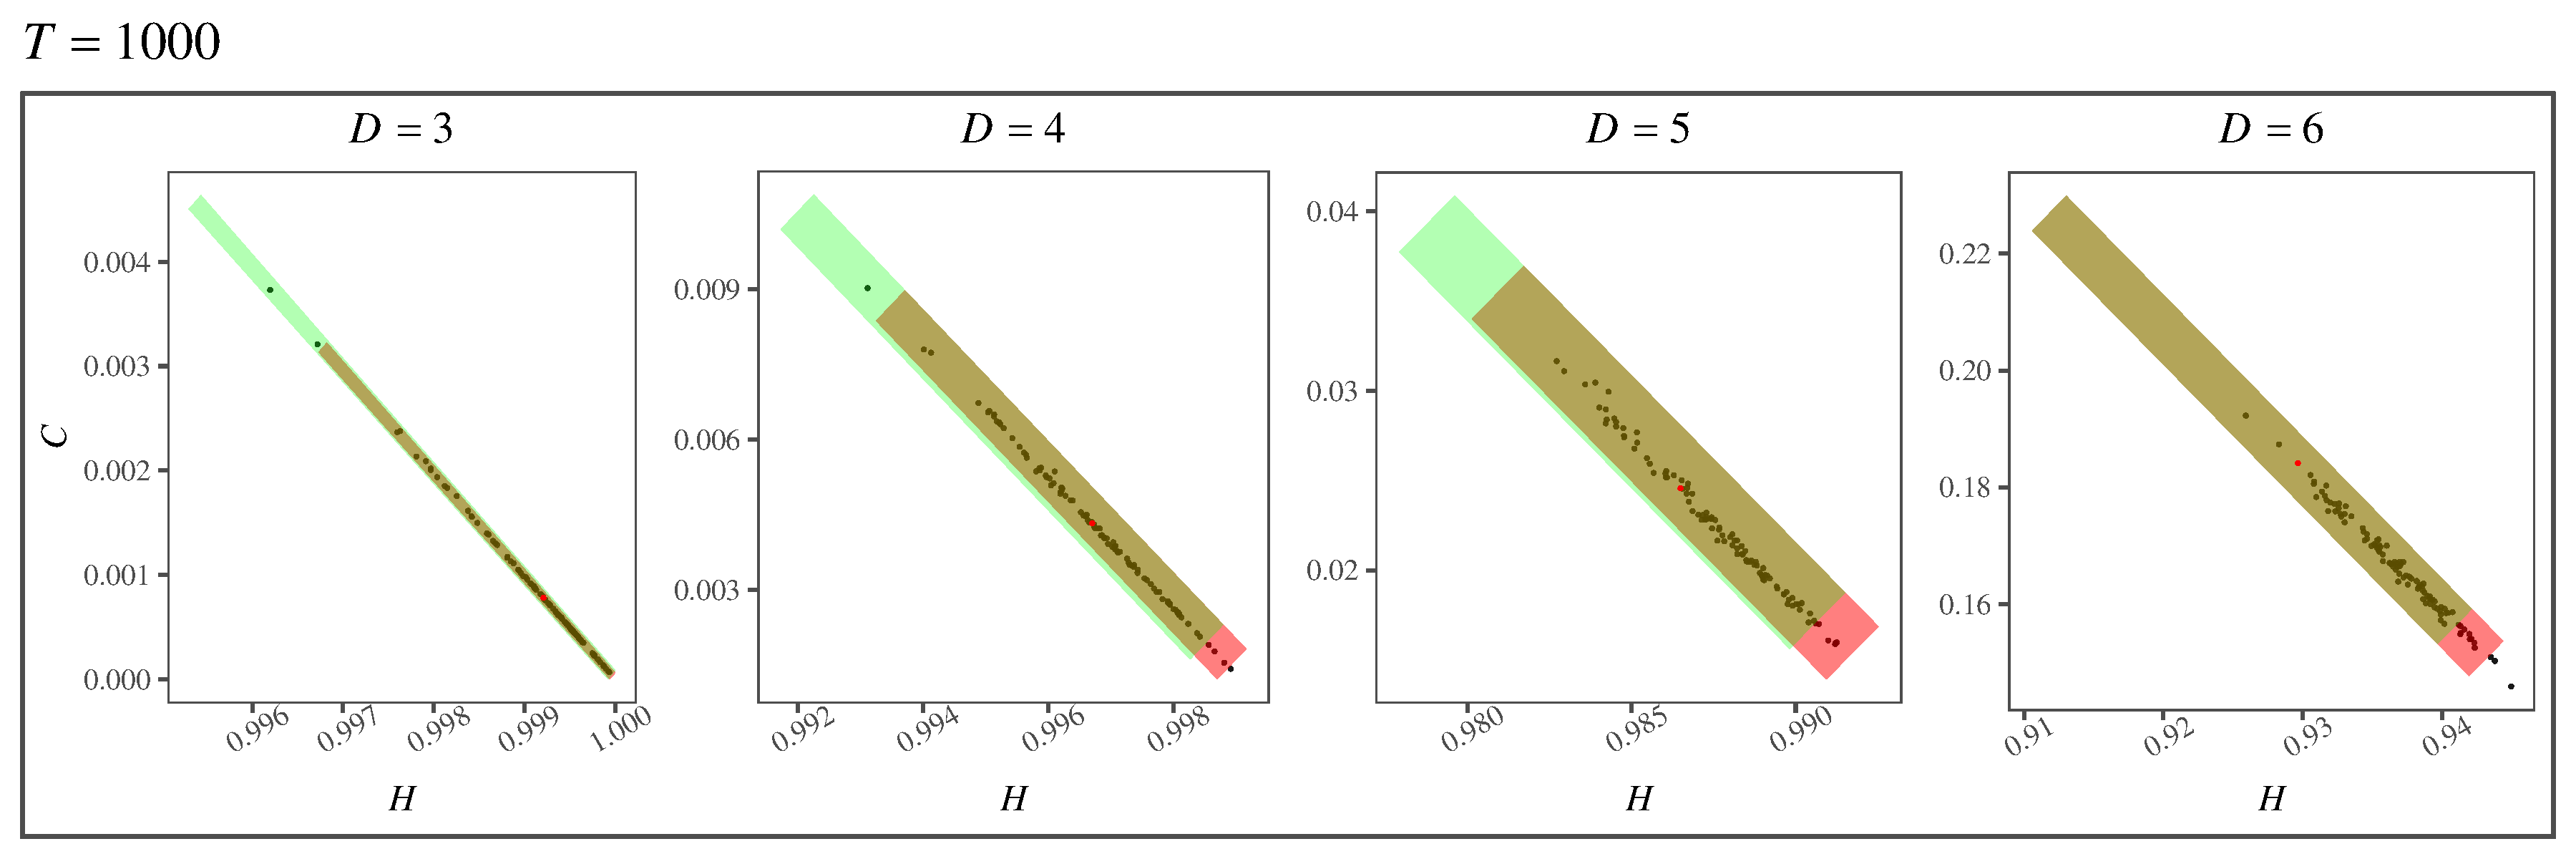
\includegraphics[width=\linewidth]{Figures/RNG-1000.pdf}
	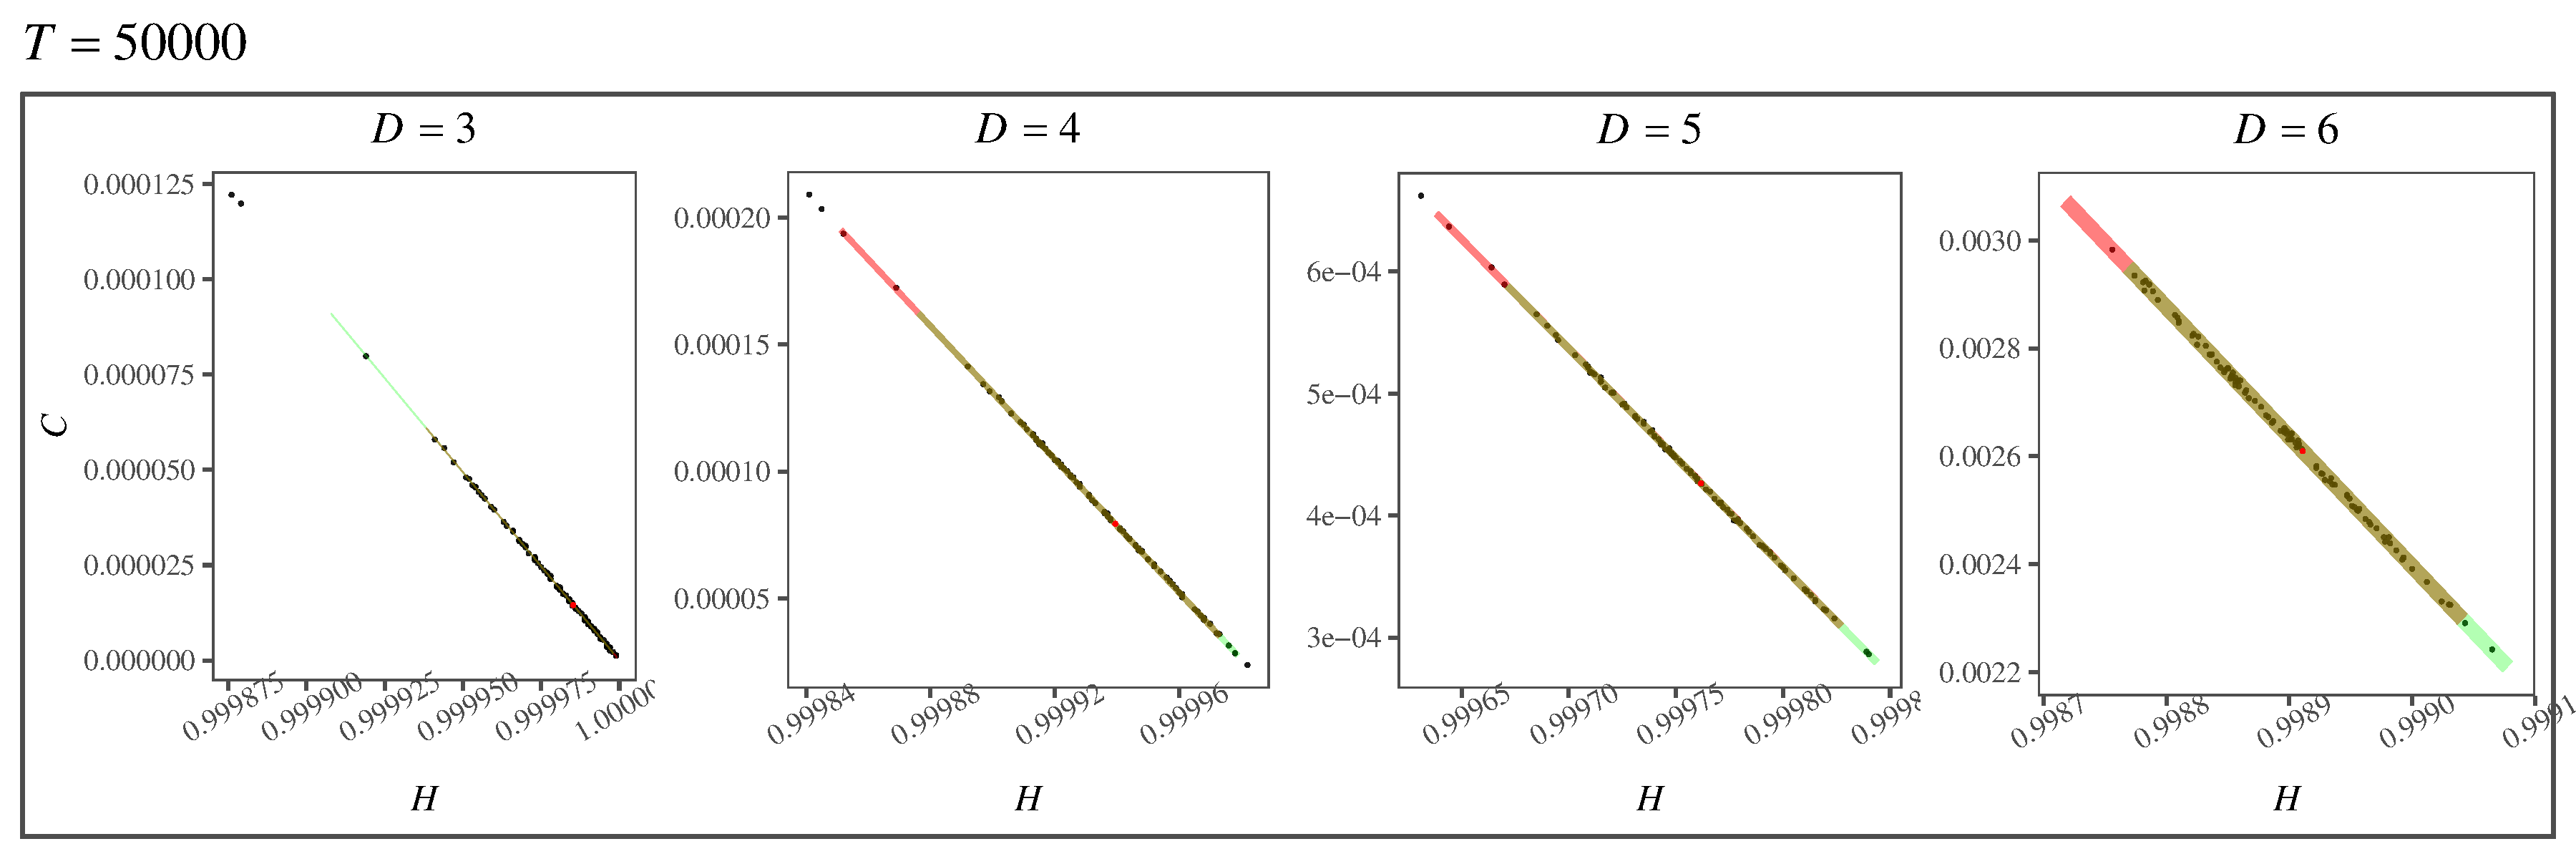
\includegraphics[width=\linewidth]{Figures/RNG-50000.pdf}
	\caption{New $100$ TRWNS and regions of confidence.}
	\label{fig:RNG}
\end{figure}

We may then conclude that the test has good empirical size, provided $D!\ll T$, a condition that does not hold for $D=6$ and $T=1000$.


\subsection{Test Power}

We assessed the power of the test by contrasting time series with different correlation structure (under the $f^{-k}$ model) in the $H \times C$ plane.
Several studies in the literature have used this approach for identifying and characterizing randomness.

Our study's basis is the emblematic time series for each length $T$ and dimension embedding $D$.
Recall that the emblematic time was chosen as the most representative of the data set.
We use these series, transform them into $f^{-k}$ correlated noise, and verify the new point's location in the $H\times C$ plane.

%Fig.~\ref{fig:CorrNoisea} illustrates the effect of a white noise time series when adding correlation structures related to the $f^{-k}$ series for $k \in \{0, 1, 2, 3 \}$.
As we can observe in the plane, as the correlation between the observations increases, that is, $k > 0$, the randomness decreases, and the entropy presented decreases, informing the loss of its stochastic characteristic.

Fig.~\ref{fig:CorrNoisea} shows the overall effect of transforming the emblematic time series into $f^{-k}$ correlated noise, with $k=1/2,1,3/2,2,5/2,3$.
At this scale, the emblematic time series $k=0$ and the one with $k=1/2$ appear overlapped.
As the correlation increases with $k$, the randomness decreases, causing a drop in the entropy; the series become progressively more predictable.

Fig.~\ref{fig:CorrNoiseb} is a zoom close to the $(1,0)$ point, along with the confidence regions for the white noise.
We see that $ k = 0 $ and $ k = 0.1 $ are inside the $\SI{95}{\percent}$ confidence region, and $ k = 0.2 $ is inside the $\SI{99}{\percent}$ box.
Notice that the time series with $k=3/10$ is outside the confidence regions and does not pass the randomness test.
The same holds for all $k>3/10$.

\begin{figure}
	\centering
	\subfloat[Points in the $H\times C$ plane of the emblematic white noise  ($k=0$) and its transformations to become $f^{-k}$ correlated noise with $k=1/2,1,3/2,2,5/2,3$.\label{fig:CorrNoisea}]{
		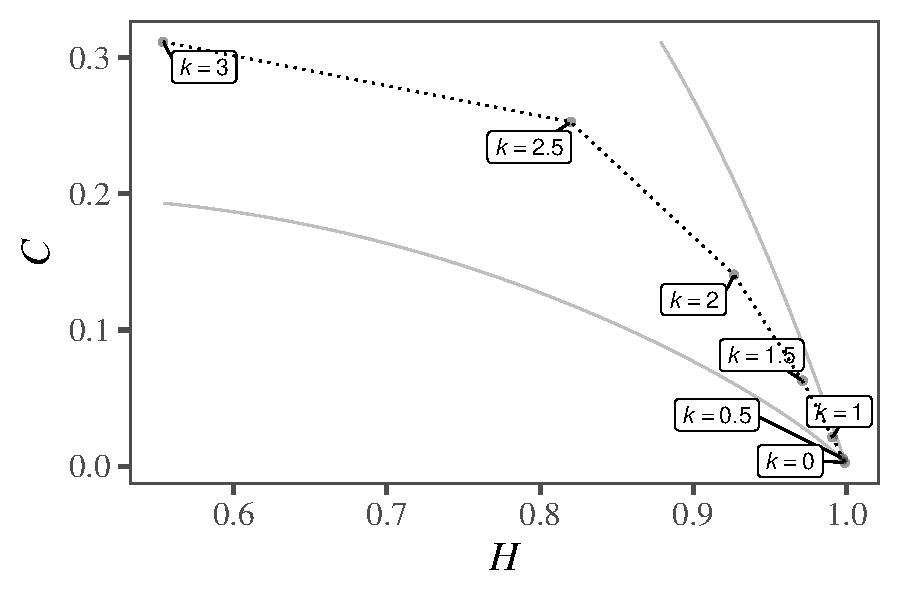
\includegraphics[width=.48\linewidth]{Figures/Correlation-Analysis-dotted.pdf}}
	\subfloat[Points of the emblematic white noise ($k=0$), and its $f^{-k}$ correlated noise versions, with $k=1/10, 1/5,3/10$ along with the confidence regions for white noise.\label{fig:CorrNoiseb}]{
		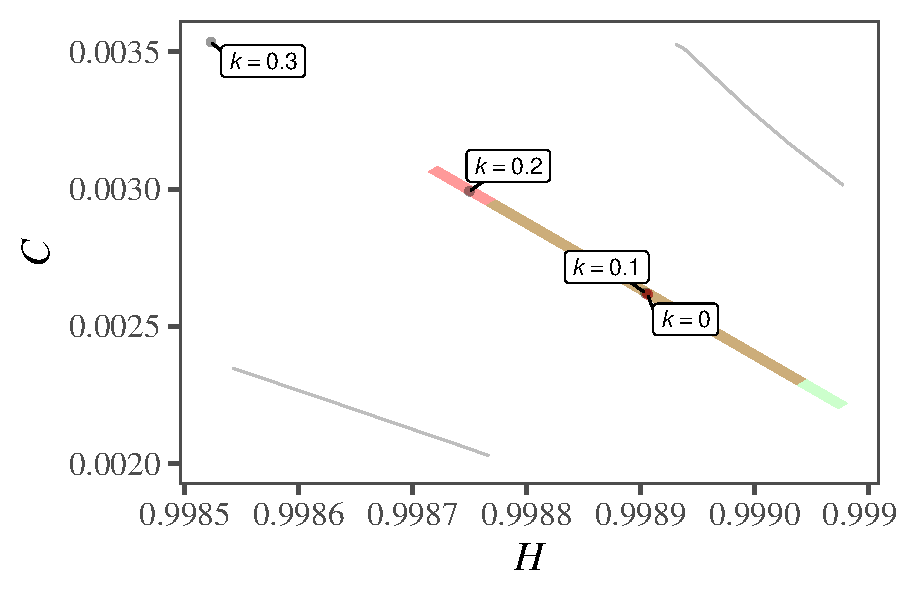
\includegraphics[width=.48\linewidth]{Figures/Correlation-Analysis-point.pdf}}
	\caption{Analysis of the test power with correlated $f^{-k}$ noise.}
	\label{fig:correlation}
\end{figure}

\subsection{Revisiting the White Noise Hypothesis in the Literature}

In this section, we compare the performance of our test with that of 
previous analyses that employ the Entropy-Complexity plane.
To this aim, we produced $100$ sequences of length $T = \num[scientific-notation=true]{5 e4}$ for each generator and computed the $p$-value for each $D = \{3, 4, 5, 6\}$.
Previous results are shown in Table~\ref{Tab:Literature}, and ours are in Table~\ref{Tab:LiteratureComparations}.
We grouped our results in those that rejected (R) the null hypothesis and those that did not reject it (NR).

\begin{table}
	\caption{Results of the sequences generated by the main PRNGs in the literature. 
		The sequences have length $T=\num[scientific-notation = true]{5 e4}$.}
	\label{Tab:LiteratureComparations}
	\centering
	\begin{tabular}{cccc}
		\toprule
		Algorithm & 
		\multicolumn{1}{c}{$D$} & 
		$p$-value &
		HC-PCA\\
		\cmidrule(lr){1-1}
		\cmidrule(lr){2-2}
		\cmidrule(lr){3-3}
		\cmidrule(lr){4-4}
		MOT & 3 & 0.305 & NR\\
		& 4 & 0.572 & NR\\ 
		& 5 & 0.455 & NR\\ 
		& 6 & 0.508 & NR\\ 
		\cmidrule(lr){1-4}
		MWC & 3 & 0.501 & NR\\
		& 4 & 0.477 & NR\\ 
		& 5 & 0.496 & NR\\ 
		& 6 & 0.496 & NR\\ 
		\cmidrule(lr){1-4}
		COM & 3 & 0.123 & NR\\
		& 4 & 0.002 & R\\ 
		& 5 & \num[scientific-notation=true]{1.11 e-16} & R\\ 
		& 6 & \num[scientific-notation=true]{1.11 e-16} & R\\ 
		\cmidrule(lr){1-4}
		LEH & 3 & 0.531 & NR\\
		& 4 & 0.515 & NR\\ 
		\bottomrule
	\end{tabular}
	\begin{tabular}{|cccc}
		\toprule
		Algorithm & 
		\multicolumn{1}{c}{$D$} & 
		$p$-value &
		HC-PCA\\
		\cmidrule(lr){1-1}
		\cmidrule(lr){2-2}
		\cmidrule(lr){3-3}
		\cmidrule(lr){4-4}
		LEH & 5 & 0.495 & NR\\ 
		& 6 & 0.501 & NR\\ 
		\cmidrule(lr){1-4}
		fGn & 3 & 0.521 & NR\\
		& 4 & 0.519 & NR\\ 
		& 5 & 0.498 & NR\\ 
		& 6 & 0.470 & NR\\
		\cmidrule(lr){1-4}
		%fBm & 3 & \num[scientific-notation=true]{1.11 e-16} & R\\ 
		%& 4 & \num[scientific-notation=true]{1.11 e-16} & R\\ 
		%& 5 & \num[scientific-notation=true]{1.11 e-16} & R\\ 
		%& 6 & \num[scientific-notation=true]{1.11 e-16} & R\\ 
		%\cmidrule(lr){1-4}
		$f^{-k}$ & 3 & 0.482 & NR\\
		& 4 & 0.520 & NR\\ 
		& 5 & 0.513 & NR\\ 
		& 6 & 0.508 & NR\\
		\cmidrule(lr){1-4}
		LCG & 3 & 0.009 & R\\ 
		& 4 & \num[scientific-notation=true]{1.11 e-16} & R\\ 
		& 5 & \num[scientific-notation=true]{1.11 e-16} & R\\ 
		& 6 & \num[scientific-notation=true]{1.11 e-16} & R\\ 
		\bottomrule
	\end{tabular}
\end{table}

Comparing Tables~\ref{Tab:Literature} and~\ref{Tab:LiteratureComparations}, we see that our test captures adequately the random dynamics of the sequences produced by most of the analyzed generators.

It is noteworthy that the generator Combo RNG sequences only pass our white noise test for $D = 3$.
In higher embedding dimensions, as we consider longer words, the sequences produced by this generator are not labeled as white noise.

